\section{\textit{Queimadas} method}

\begin{frame}
  \textit{Queimadas} method
\end{frame}

\subsection{\textit{Queimadas} method to forecast}

\begin{frame}
  \frametitle{\textit{Queimadas} method for forecasting heat foci}
  \begin{enumerate}
    \item Get time series of two reference satellites:
    \begin{itemize}
      \item One which we would like to extend in time (A.K.A. $y$).
      \item The other one covering the whole time line we would like to
      forecast (A.K.A. $x$).
    \end{itemize}
    \item Adjust a linear model ($y = Ax + b$) to the overlapping observations
    in the time series of two reference satellites, using only the month of the
    observations.
    \item Use the model to predict the whole time line.
    \item Check forecast results.
  \end{enumerate}
\end{frame}

\begin{frame}
  \frametitle{Linear model NOAA-12 vs. AQUA\_M-T}
  \begin{figure}
    \centering
    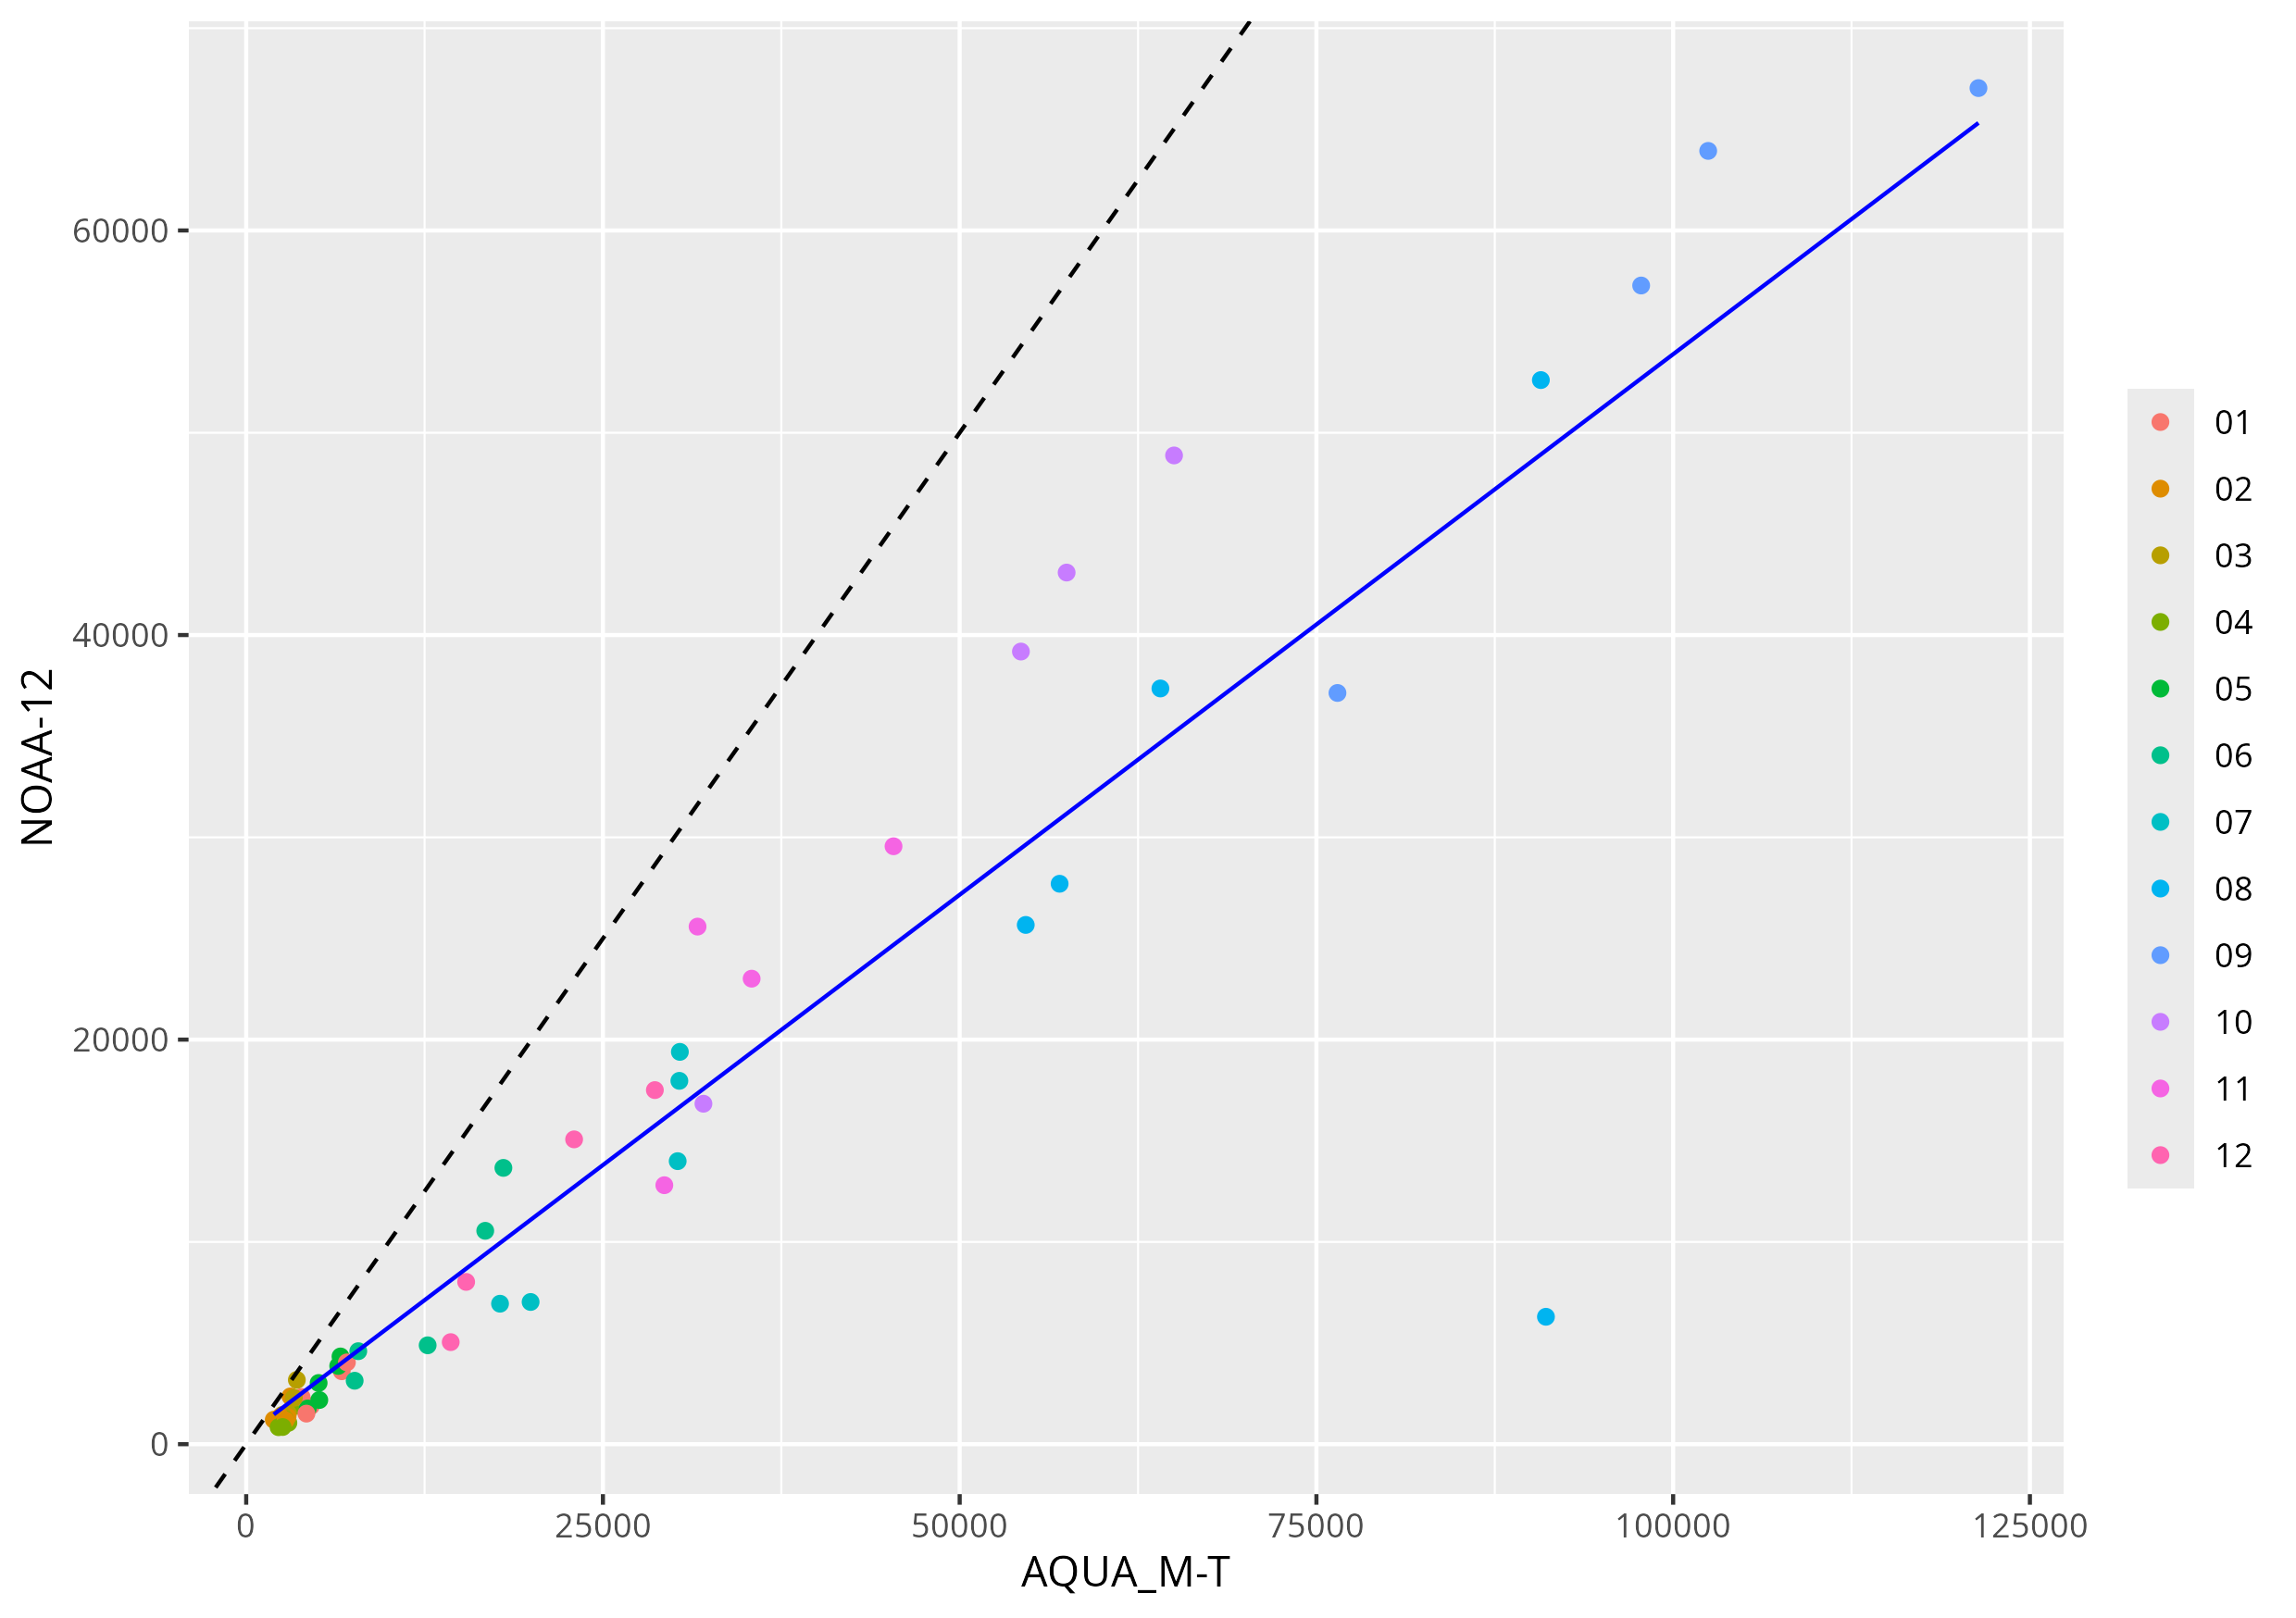
\includegraphics[scale=0.5]
    {figures/plot_queimadas_lm_NOAA-12_along_AQUA_M-T.png}
  \end{figure}
\end{frame}

\begin{frame}
  \frametitle{Linear model NPP-375D vs. AQUA\_M-T}
  \begin{figure}
    \centering
    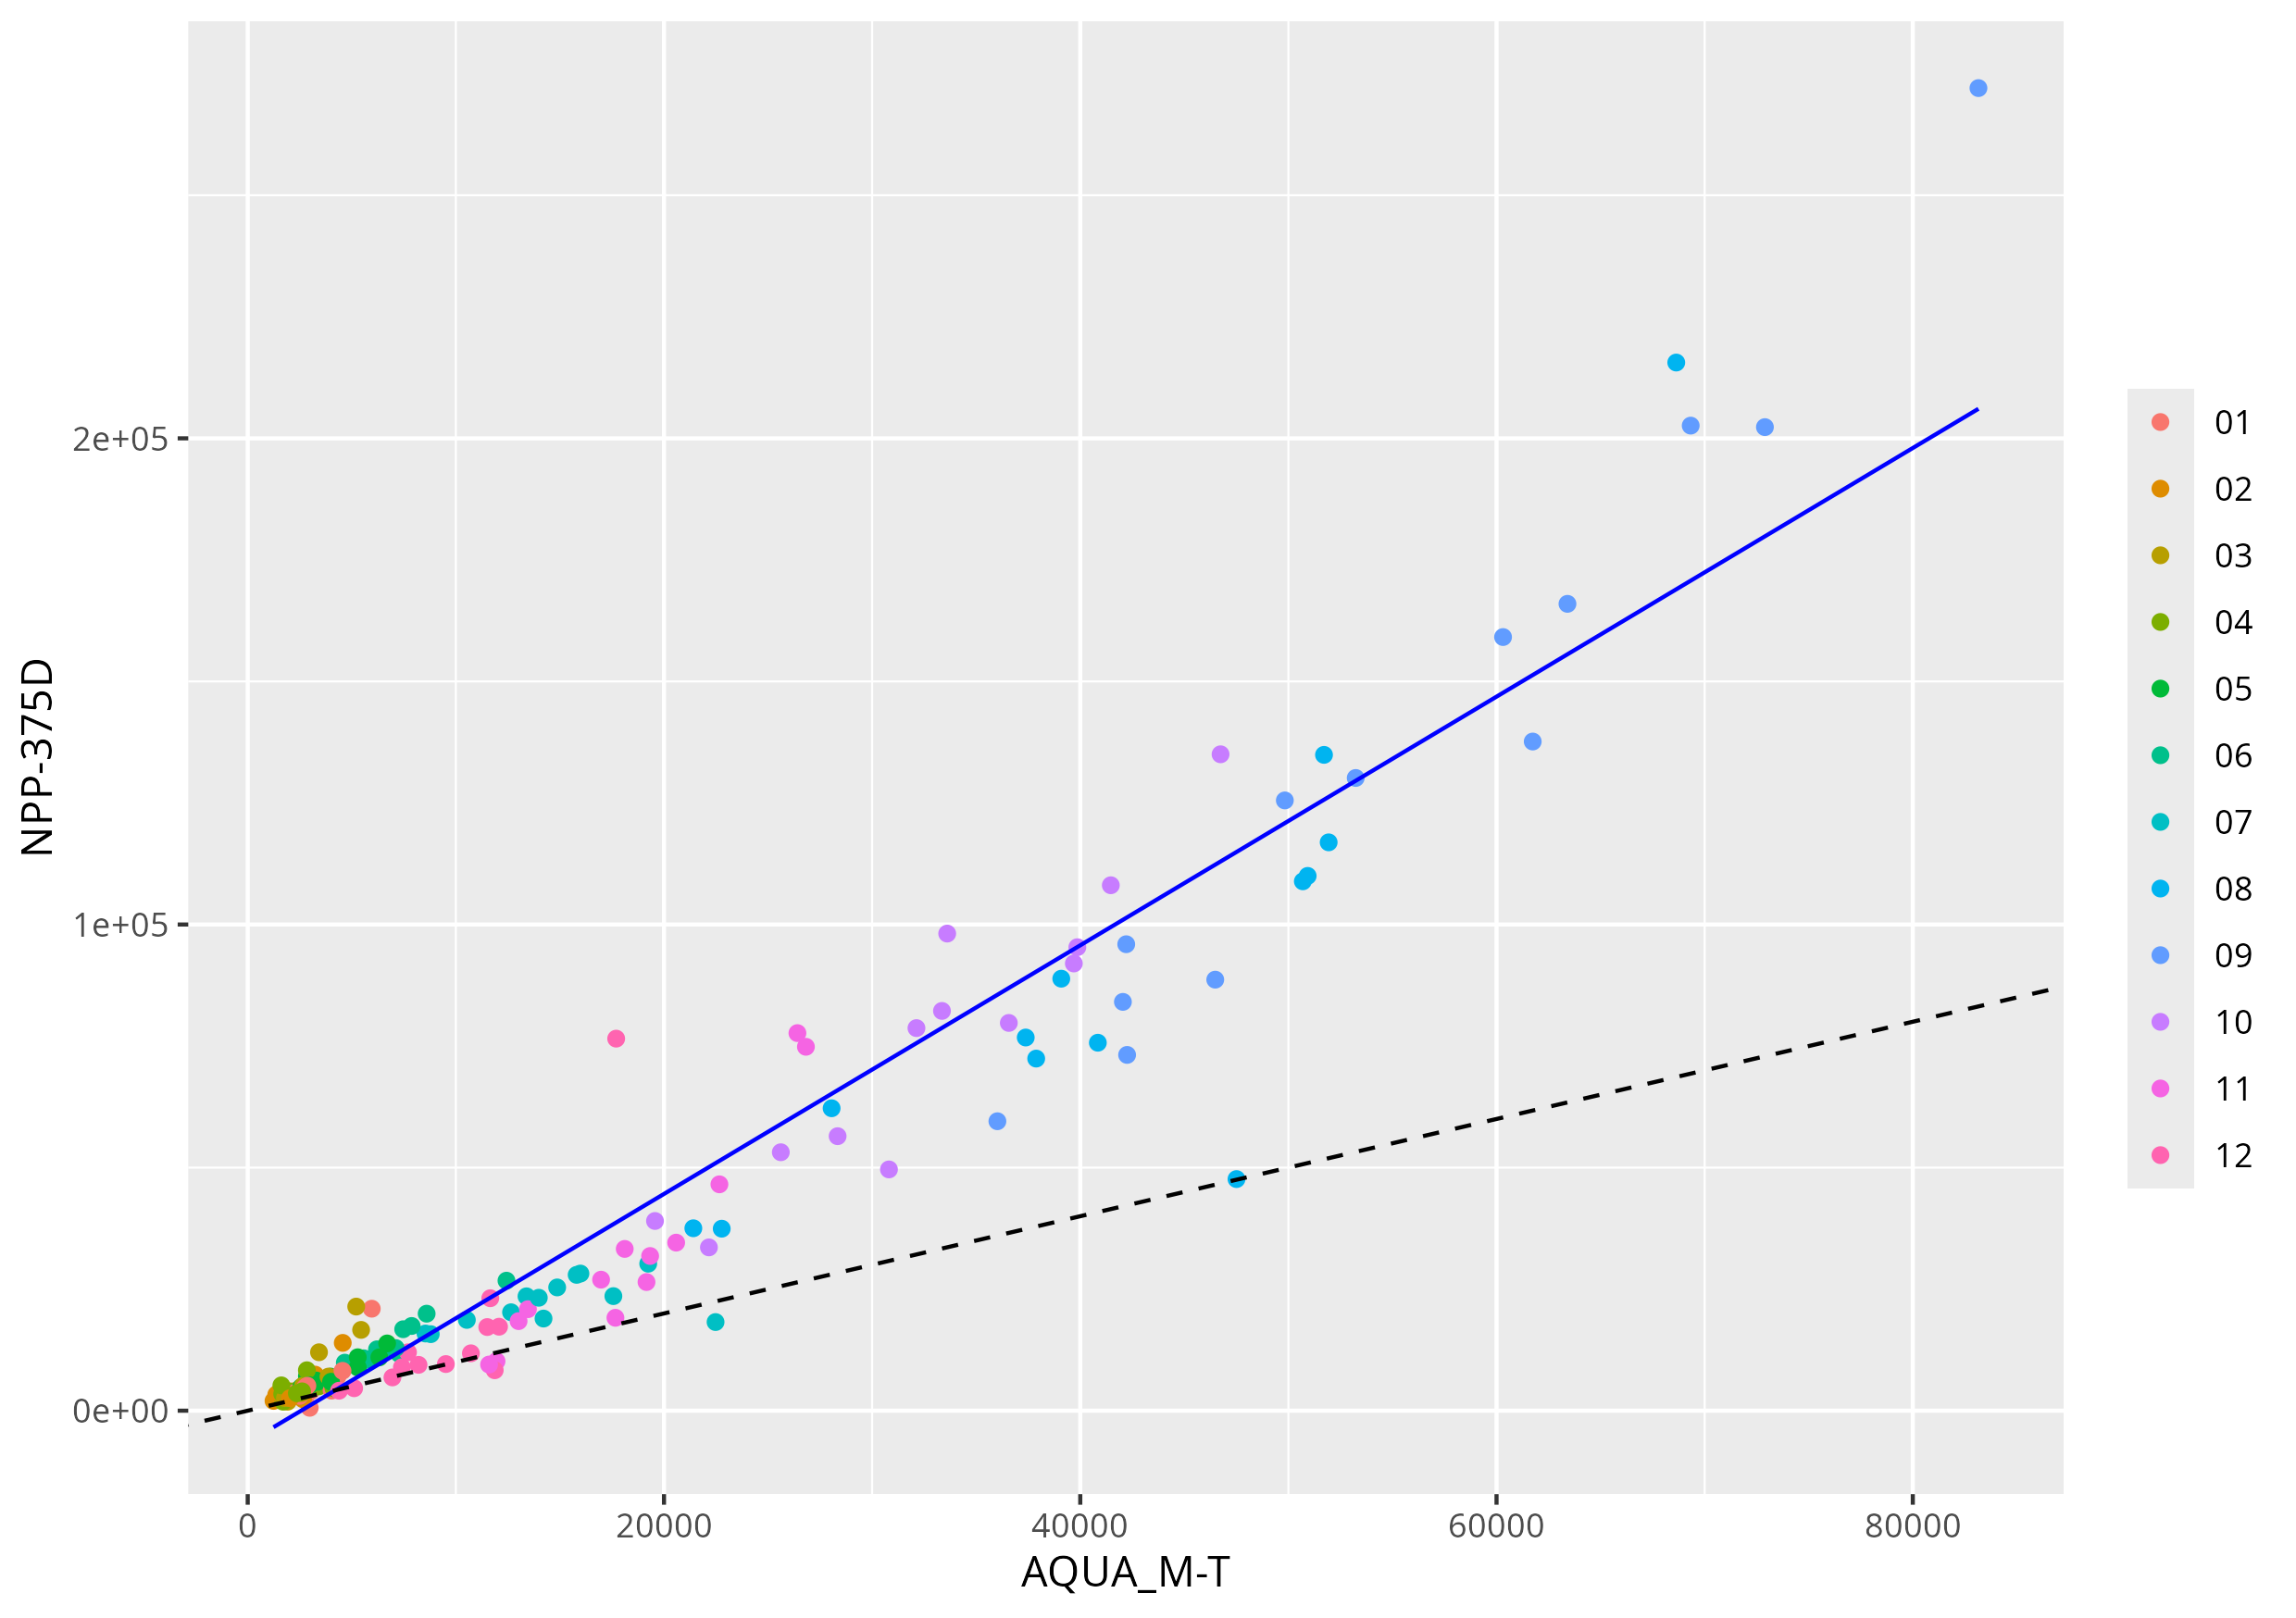
\includegraphics[scale=0.5]
    {figures/plot_queimadas_lm_NPP-375D_along_AQUA_M-T.png}
  \end{figure}
\end{frame}

\begin{frame}
  \frametitle{Linear model NPP-375-PM vs. AQUA\_M-T}
  \begin{figure}
    \centering
    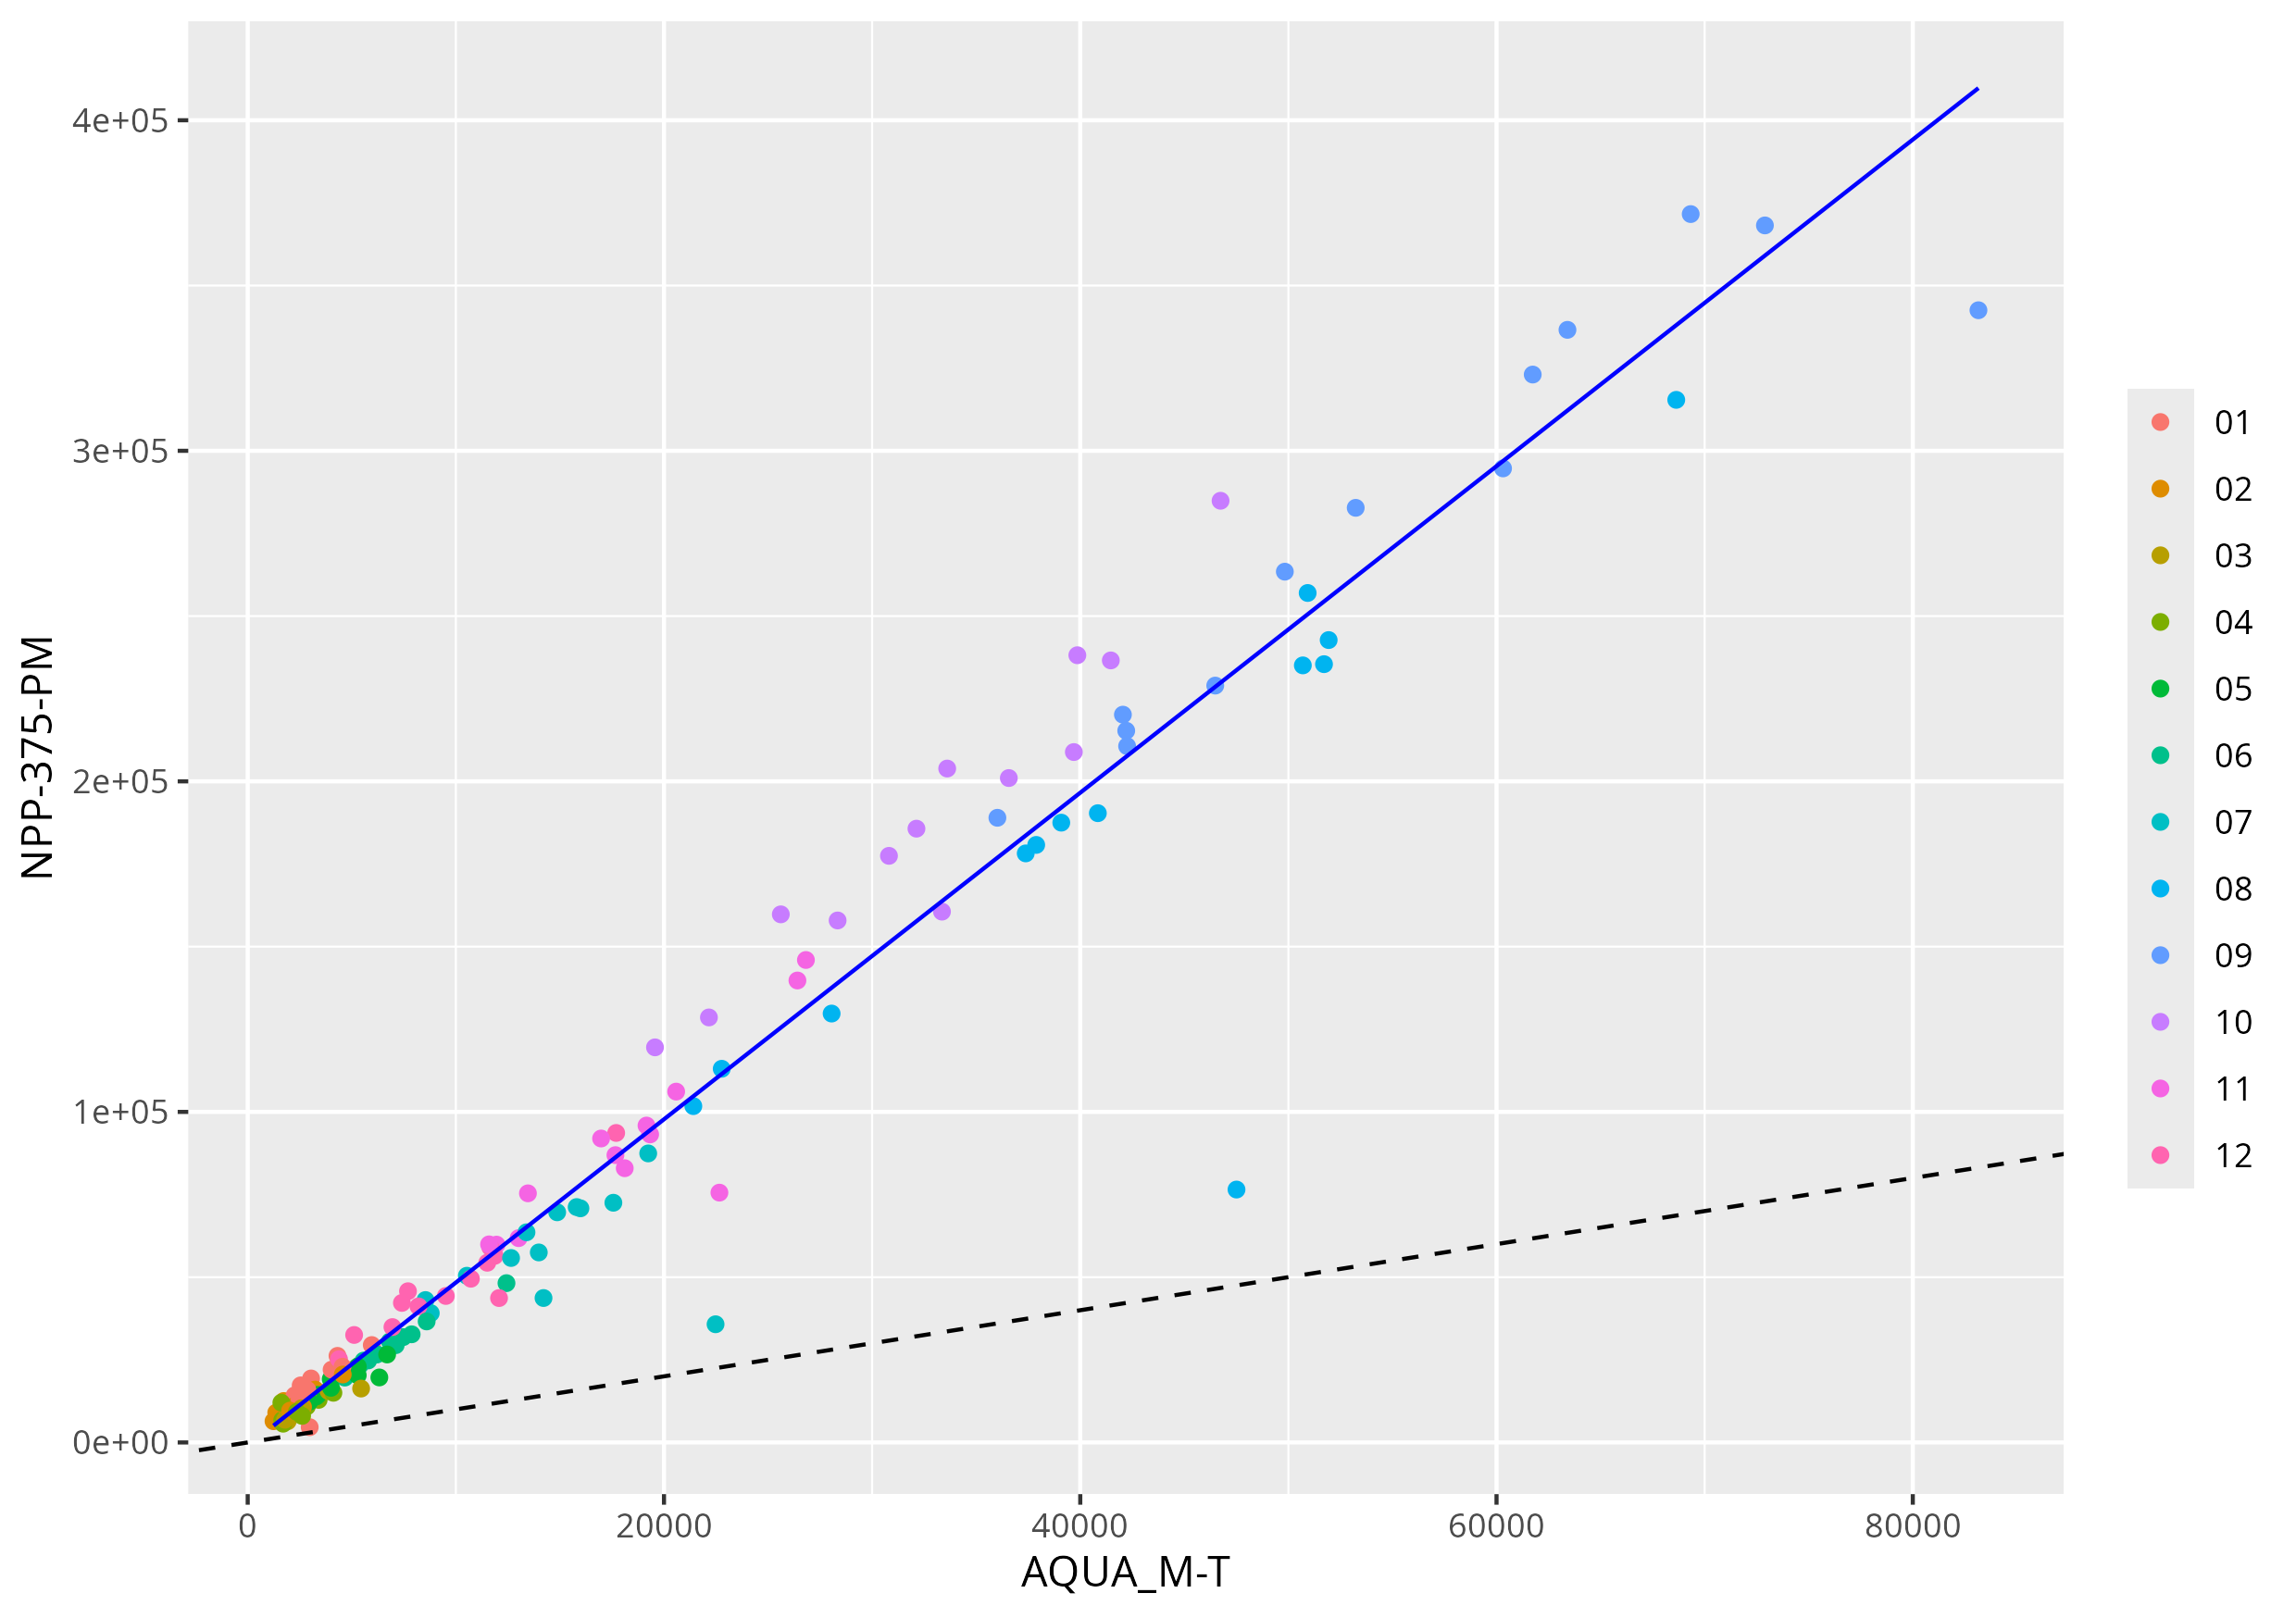
\includegraphics[scale=0.5]
    {figures/plot_queimadas_lm_NPP-375-PM_along_AQUA_M-T.png}
  \end{figure}
\end{frame}

\begin{frame}
  \frametitle{Linear regression parameters}
    \centering
    \csvautotabular{tables/queimadas_method_lm_equation.csv}
\end{frame}

\begin{frame}
  \frametitle{Stretch NOAA-12 to match AQUA\_M-T}
  \begin{figure}
    \centering
    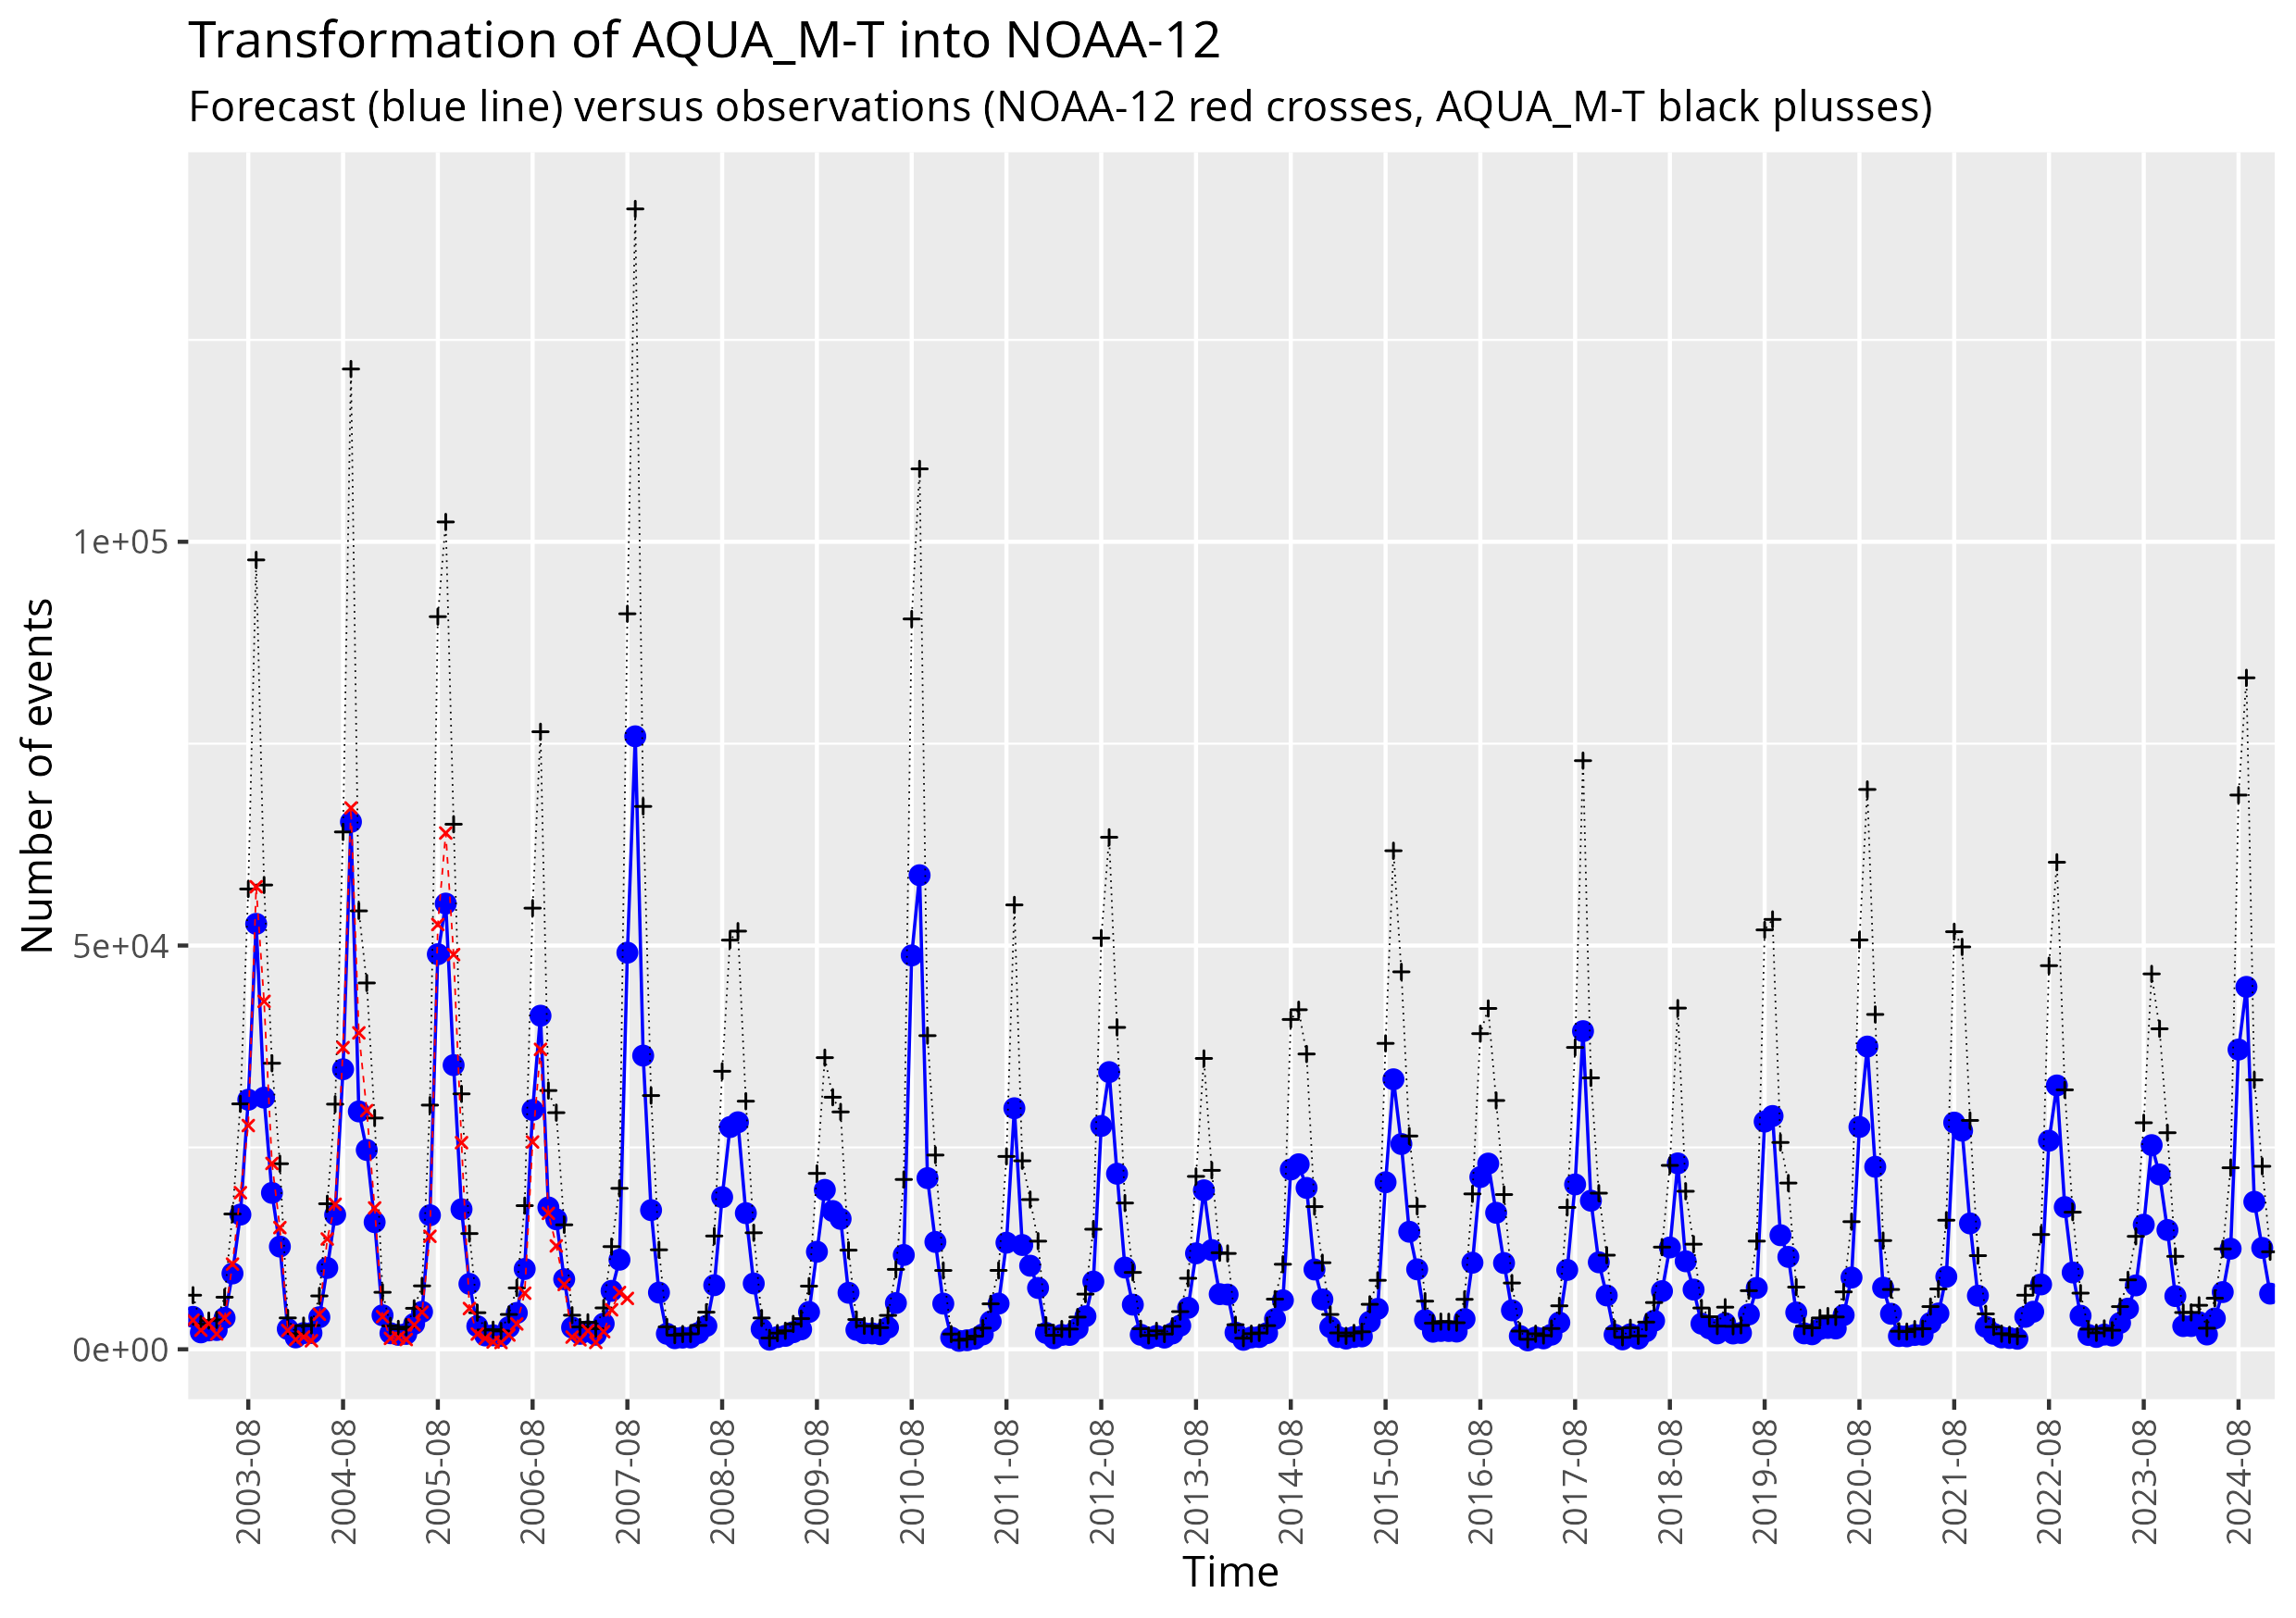
\includegraphics[scale=0.5]
    {figures/plot_forecast_NOAA-12_along_AQUA_M-T.png}
  \end{figure}
\end{frame}

\begin{frame}
  \frametitle{Stretch NPP-375D to match AQUA\_M-T}
  \begin{figure}
    \centering
    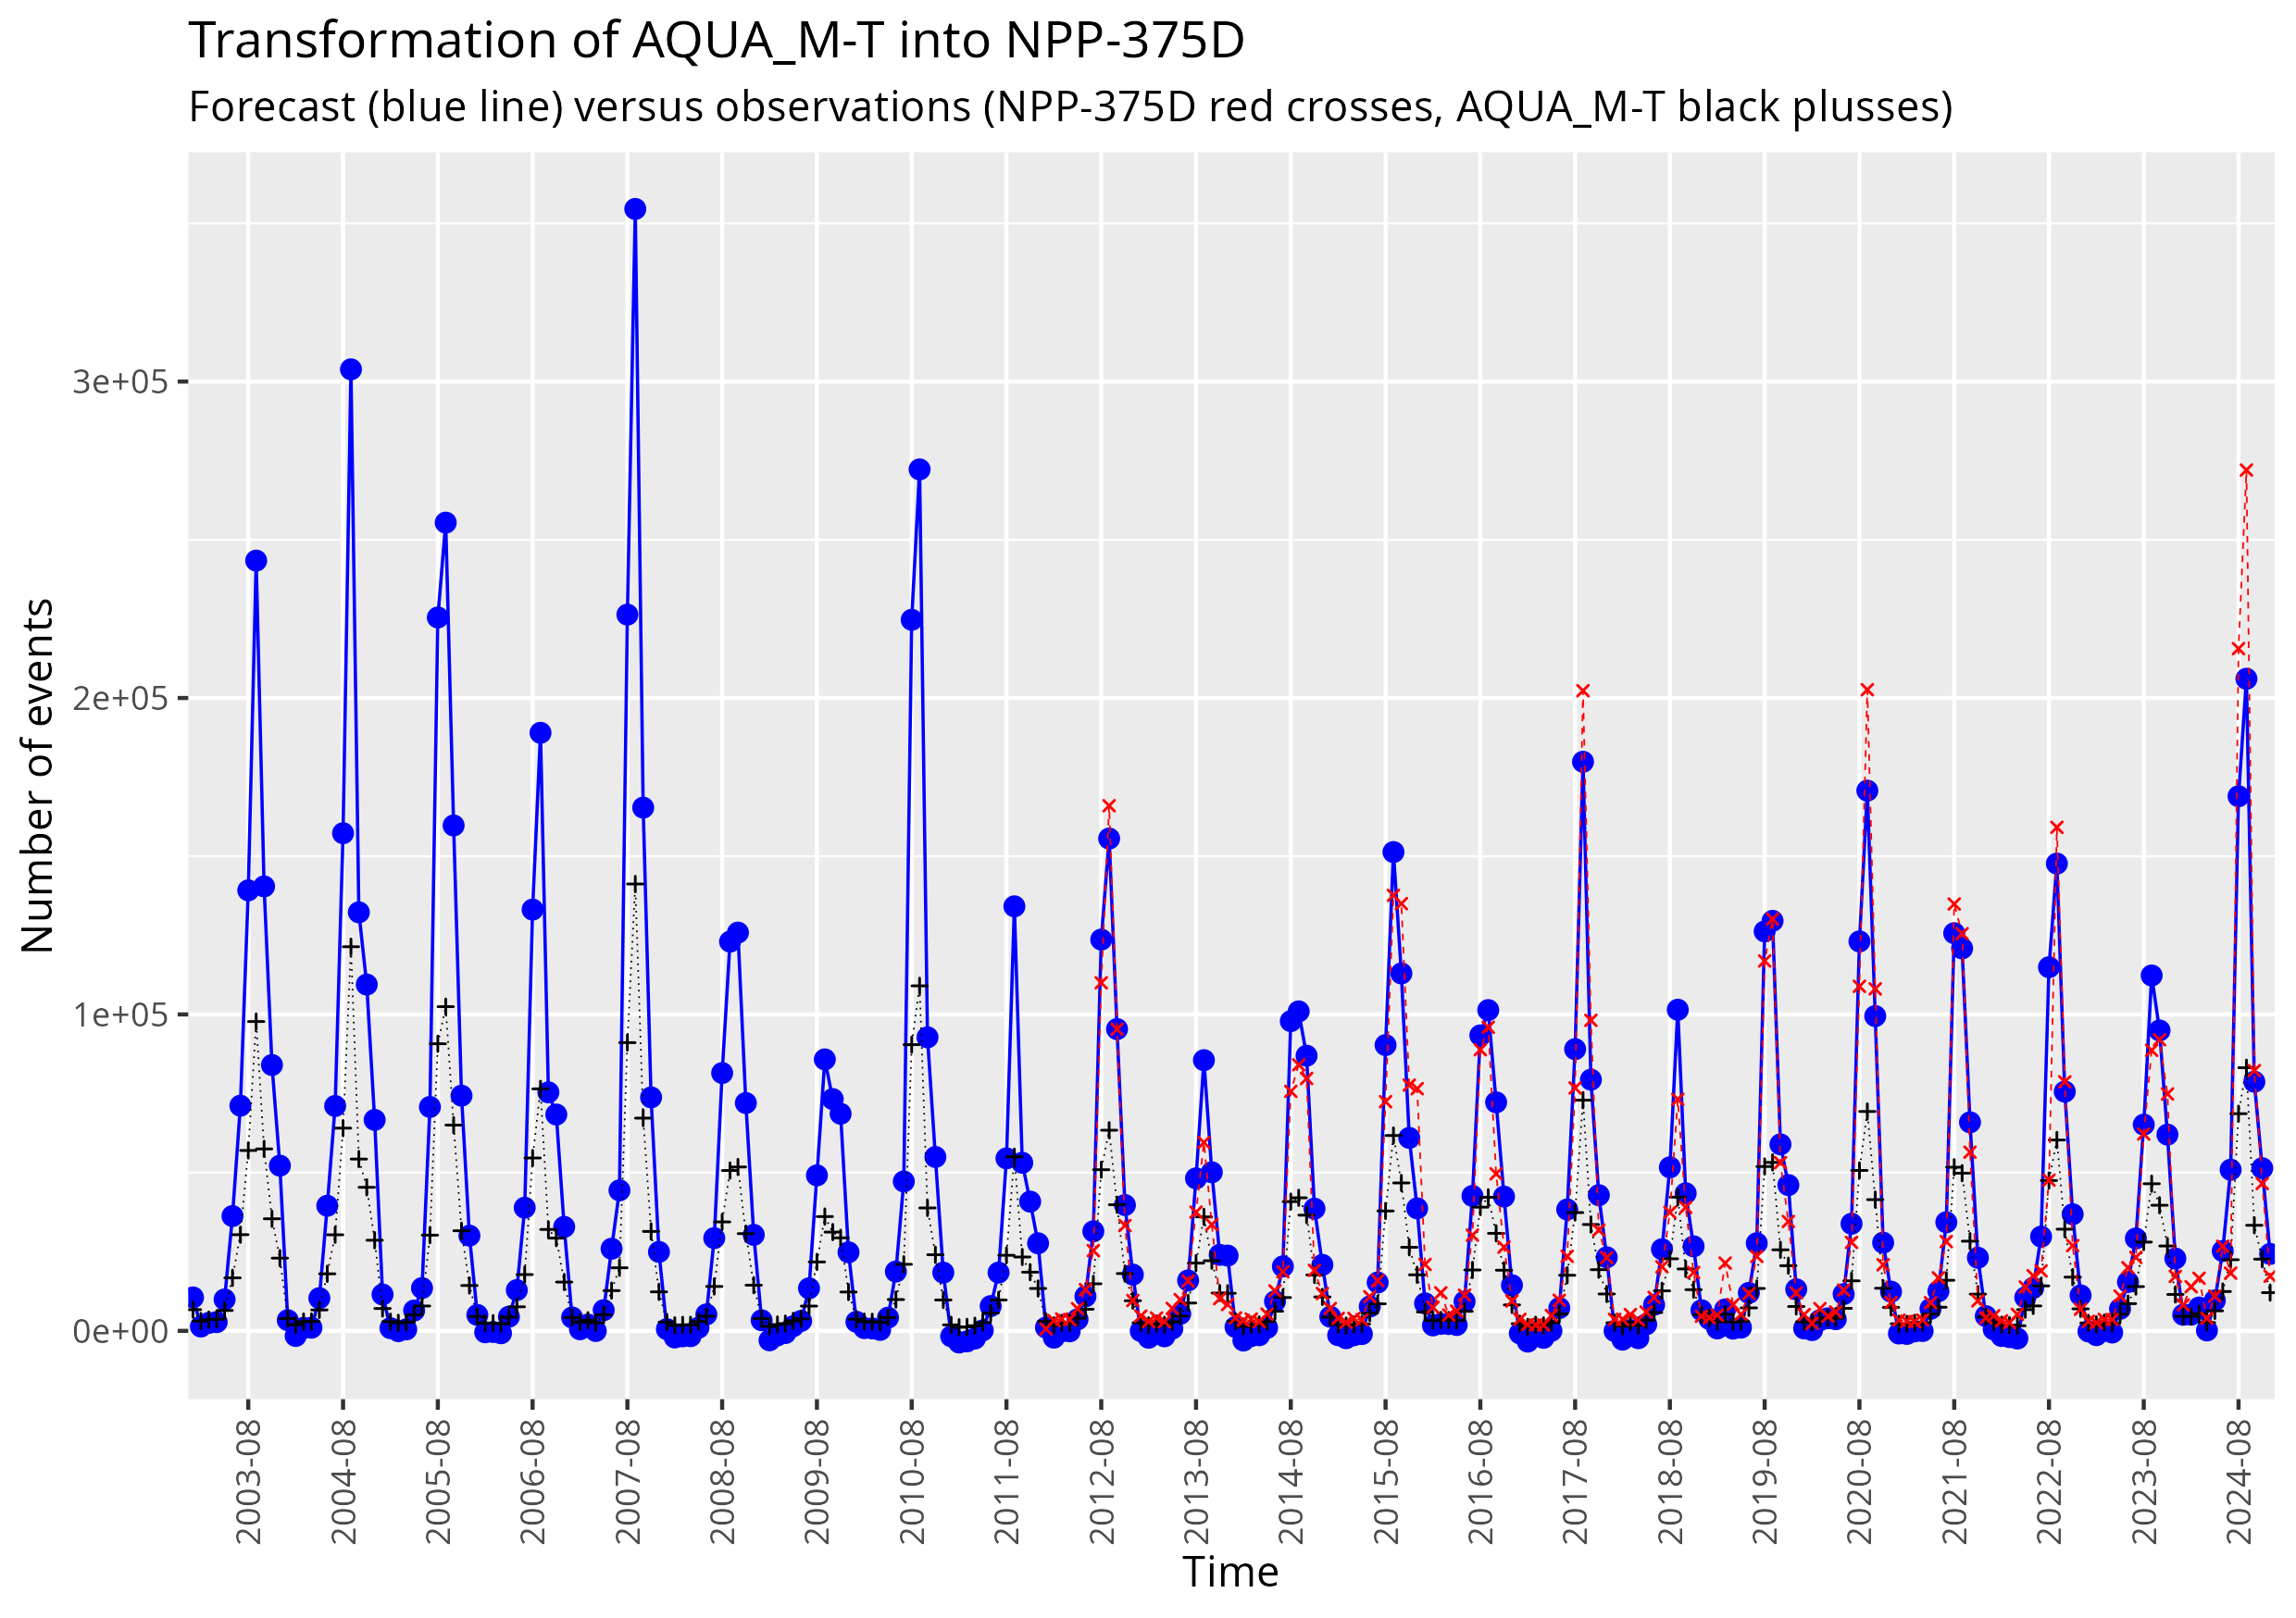
\includegraphics[scale=0.5]
    {figures/plot_forecast_NPP-375D_along_AQUA_M-T.png}
  \end{figure}
\end{frame}

\begin{frame}
  \frametitle{Stretch NPP-375-PM to match AQUA\_M-T}
  \begin{figure}
    \centering
    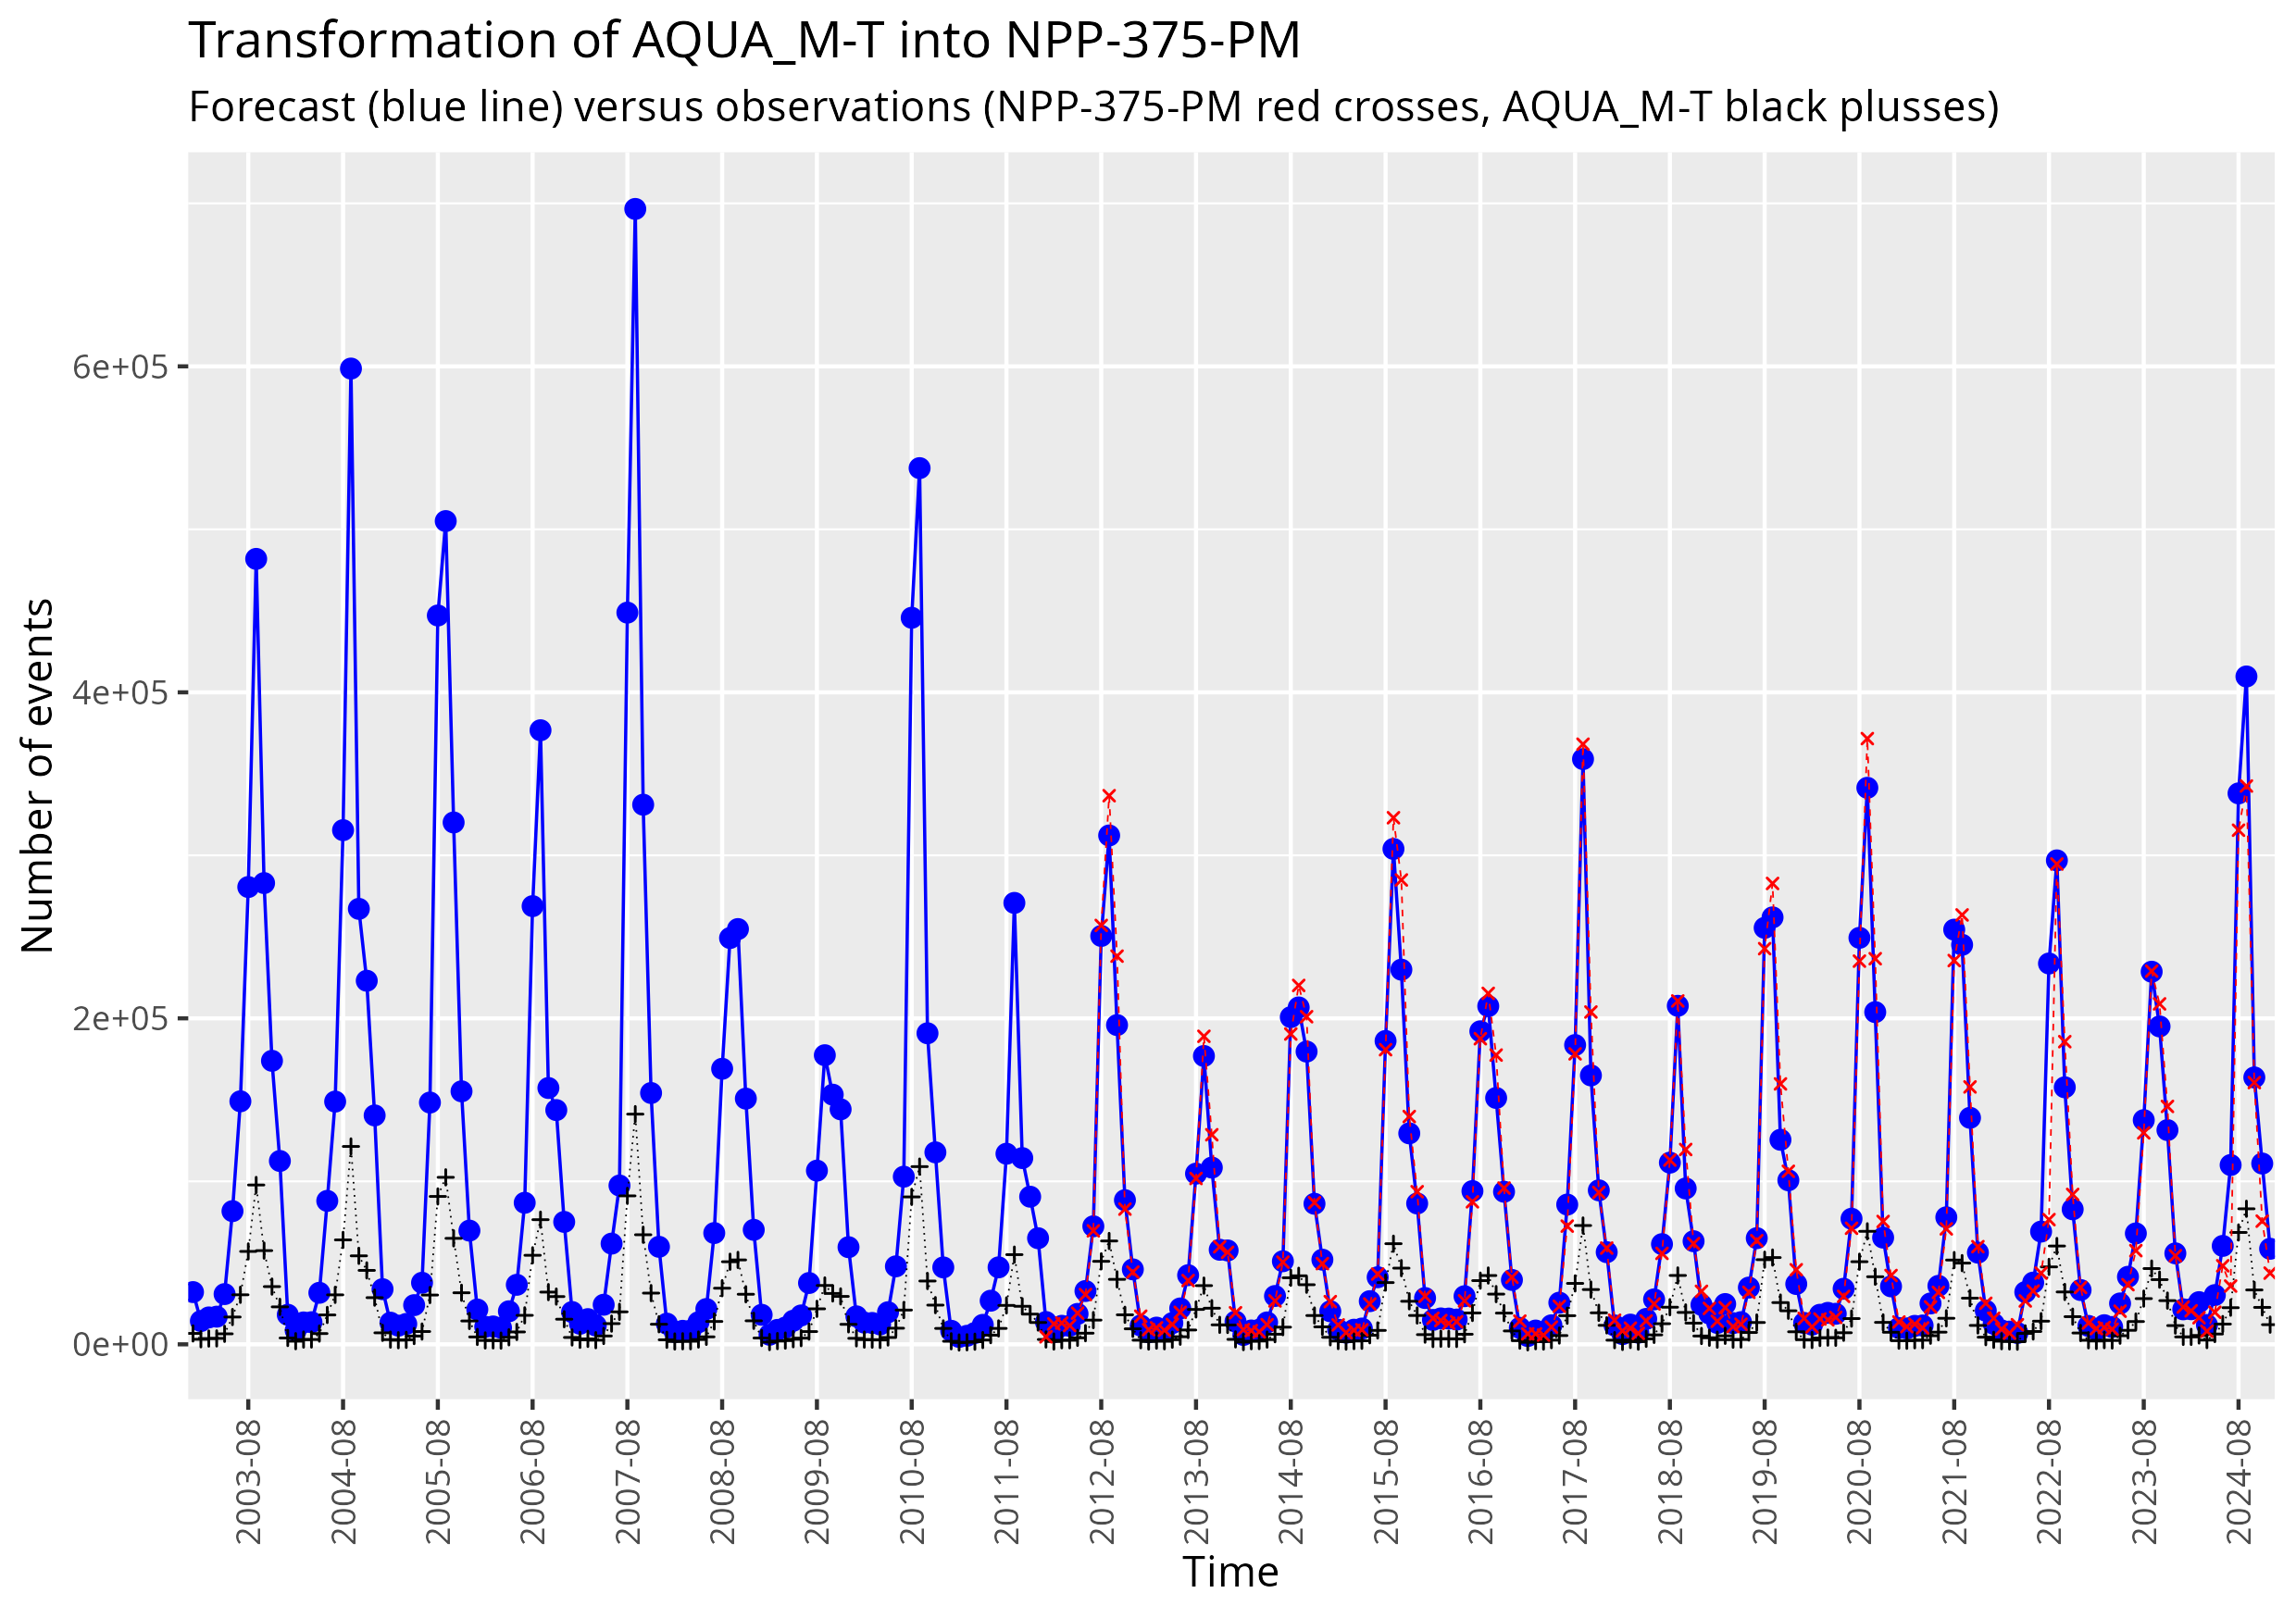
\includegraphics[scale=0.5]
    {figures/plot_forecast_NPP-375-PM_along_AQUA_M-T.png}
  \end{figure}
\end{frame}

